\documentclass[11pt]{article}

\usepackage{fullpage}
\usepackage{graphicx}
\usepackage{amsfonts}
\usepackage{amsmath}

\begin{document}

\author{Fahim Yusufzai}
\title{An Equation a Day Keeps Friends Away}
\date{\today}
\maketitle
\pagebreak

\begin{center}
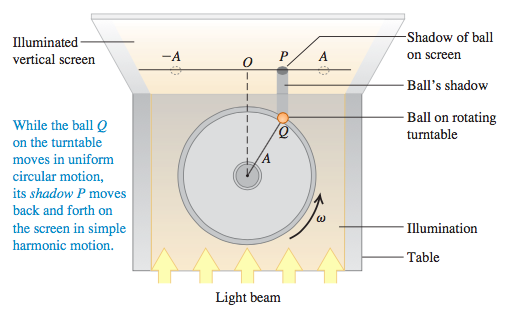
\includegraphics[scale=0.5]{demo}
\end{center}
We begin this section by recalling the basic wave eqution 
$v = f \lambda$ and simple adaptions of periodic motion;
namely Hooke's Law and how we can describe an object undergoing periodic 
motion (contstrained by small displacement) in the following approach:
	\begin{eqnarray}
	v = 2 \pi r f \\
	\dfrac{v}{r} = \dfrac{d \theta}{dt} = \omega = 2 \pi f \\ 
	\dfrac{d^2x(t)}{dt^2} = a(t) = \omega^2x(t) 
	\textrm{ where } x(t) \leq r\\
	\dfrac{d^2x(t)}{dt^2} = \dfrac{F}{m} = -\dfrac{k}{m} x(t)
	 =  \omega^2x(t) \\
	\dfrac{d^2}{dt^2} \sin(\omega t) = - \omega^2 \sin(\omega t) \\
	\omega^2 = \dfrac{k}{m} \\
	x(t) = c \sin (\omega t + \phi) \\
	-c \leq x(t) \leq c \\
	c = \textrm{amplititude} = r = A
	\end{eqnarray}

Putting this all together we get the following: 
	\begin{eqnarray}
	x(t) = A \sin (\omega t + \phi) \\
	\dfrac{dx(t)}{dt} = v(t) = A\omega \cos (\omega t + \phi) \\
	\dfrac{d^2x(t)}{dt^2} = a(t) = -A\omega^2 \sin (\omega t + \phi) \\
	\end{eqnarray}

We then note the following relationship:
	\begin{equation}
	 x^2(t) + \dfrac{v^2(t)}{\omega^2} =
	 A^2(\sin ^2 (\phi) +\cos ^2 (\phi)) = A^2
	\end{equation}

\pagebreak

We know derive a basic equivalence principle for the \textsl{total energy} 
of a system:

	\begin{equation}
	E = \frac{1}{2}mv^2 + \frac{1}{2} kx^2 =
	\frac{1}{2} \left[ m \omega^2 A^2 \cos^2 (\phi) + kA^2 \sin^2 (\phi) \right] = 
	\frac{1}{2} \left[ kA^2 \left( \cos^2 (\phi) + \sin^2 (\phi) \right) \right] = 	
	\frac{1}{2} kA^2
	\end{equation}
	
So far we have modelled simple periodic motion in 
a 1-dimensional setting; with slight modifcations we can generalize
our model to describe simple harmonic motion under different sources
of restoring forces (gravity for example).
We will now extend our analysis of periodic motion to a 2-dimensional 
setting and describe the height of a wave given its 1-dimensional 
displacement and time.

\begin{center}
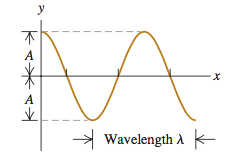
\includegraphics[scale=0.6]{wave1}
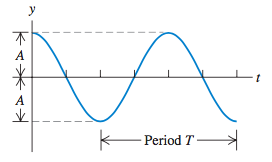
\includegraphics[scale=0.6]{wave2}
\end{center}

	\begin{eqnarray}
	\left. y(x,t) \right|_{x=0} = A \cos(\omega t) \\
	y(x,t) = A \cos(\omega \left( t - \dfrac{x}{v} \right)) \\
	y(x,t) = A \cos(2 \pi f \left( \dfrac{x}{v} - t \right)) \\
	y(x,t) = A \cos(2 \pi \left( \dfrac{x}{\lambda} - \dfrac{t}{T} \right)) \\	
	\lambda = \dfrac{2 \pi}{k} \textrm{ where $k$ = wave number} \\
	y(x,t) = A \cos( kx - \omega t) \\	
	\dfrac{d}{dt}(kx - \omega t) = 0 \Rightarrow
	\dfrac{dx}{dt} = \dfrac{\omega}{k} = v
	\end{eqnarray}

Once more, putting this all together we have the following:
	\begin{eqnarray}
	\dfrac{\partial^2 y(x,t)}{\partial x^2} = -Ak^2 \cos(kx - \omega t) =
	-k^2 y(x,t) \\
	\dfrac{\partial^2 y(x,t)}{\partial t^2} = -A\omega^2 \cos(kx - \omega t) =
	-\omega^2 y(x,t)
	\end{eqnarray}
	
We then note the following relationship:
	\begin{equation}
	\dfrac{\partial^2 y(x,t) / \partial x^2}{\partial^2 y(x,t) / \partial t^2} =
	\dfrac{k^2}{\omega^2}	= \dfrac{1}{v^2} 
	\textrm{ where $v$ = the speed at which the wave propagates}
	\end{equation}

\pagebreak

\begin{center}
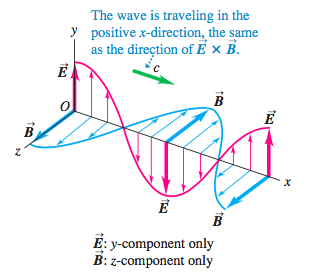
\includegraphics[scale=0.7]{emwaves}
\end{center}
This leads us exactly to our desired result, The Universal Wave Equation:

	\begin{equation}
	\dfrac{\partial^2 y(x,t)}{\partial x^2} 
	=  \dfrac{1}{v^2} \dfrac{\partial^2 y(x,t)}{\partial t^2} 
	\end{equation}

\end{document}